\documentclass{beamer}

\usepackage{comment}
\usepackage{color}
\usepackage{listings}
\usepackage{verbatim}
\usepackage{multicol}
\usepackage{booktabs}
\usepackage{textpos}
\usepackage{graphicx}
\usepackage{graphics}
\definecolor{green}{RGB}{0,128,0}

\newcommand\gehcomment[1]{{{\color{orange} #1}}}
\newcommand\add[1]{{{\color{blue} #1}}}
\newcommand\remove[1]{\sout{{\color{red} #1}}}
\newcommand\codecomment[1]{{{\color{green} #1}}}
\newcommand\redcomment[1]{{{\color{red} #1}}}
\newcommand\bluecomment[1]{{{\color{blue} #1}}}
\newcommand\greencomment[1]{{{\color{green} #1}}}
\newcommand\magentacomment[1]{{{\color{magenta} #1}}}

\begin{document}
\title{Radial CO2 Injection\ldots}
\author{Michael Nole}
\date{\today}

%\frame{\titlepage}

%-----------------------------------------------------------------------------
\section{Description of Radial CO2 Injection Scenario}

\subsection{Radial CO2 Injection Conceptual Model}

\frame{\frametitle{Description of Radial CO2 Injection Scenario}

The ``Radial CO2 Injection Scenario'' simulates 1D, radial injection of supercritical CO2 into an aquifer. This scenario demonstrates the basics of setting up input decks using \bluecomment{SCO2 MODE}. The base example models isothermal injection into a fresh water aquifer. Subsequent variants add a salt component and non-isothermal effects.

This demonstration covers the following:

\begin{itemize}
  \small
  \item Set up a 1D, isothermal cylindrical CO2 injection using SCO2 mode.
  \item Run the simulation, visualize results.
  \item Modify initial and boundary conditions to simulate injection into a saline aquifer.
  \item Run the simulation, visualize results.
  \item Modify initial and boundary conditions to simulate non-isothermal injection into a saline aquifer.
  \item Run the simulation, visualize results.
\end{itemize}
}

%-----------------------------------------------------------------------------
\section{Description of Input Deck}

%-----------------------------------------------------------------------------
\subsection{DESCRIPTION}

\begin{frame}[fragile]\frametitle{DESCRIPTION}

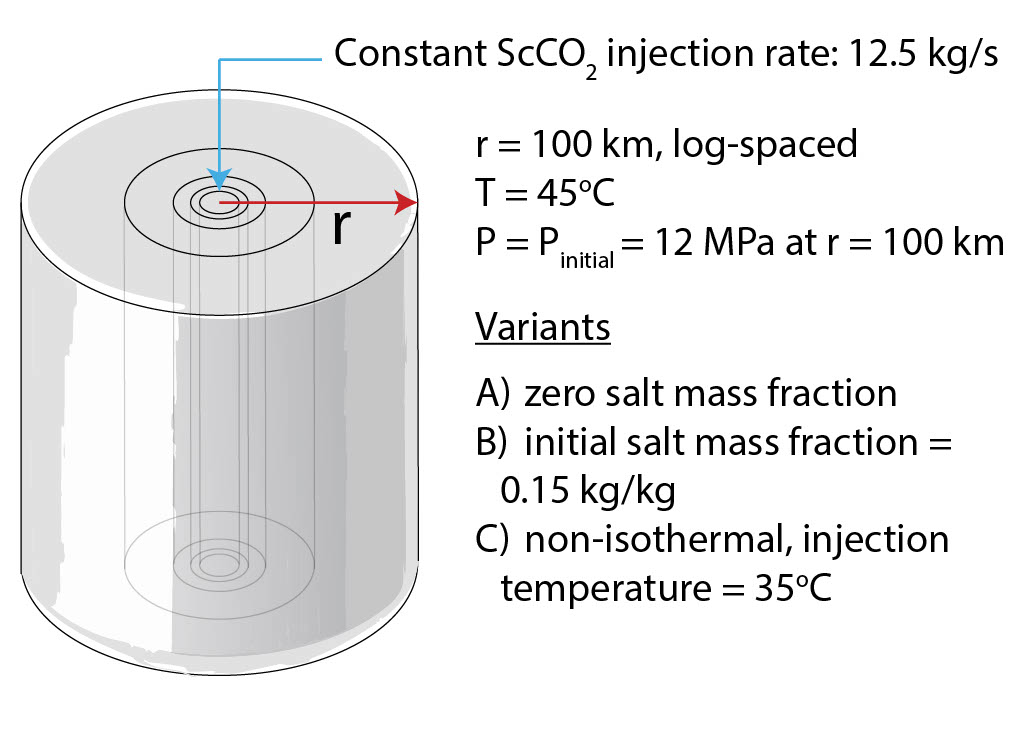
\includegraphics[height=3in]{radial_inj_fig.jpg}

\end{frame}

%-----------------------------------------------------------------------------
\subsection{SIMULATION\_RADIAL-INJECTION-NO-SALT}

\begin{frame}[fragile]\frametitle{SIMULATION: Radial Injection (No Salt)}

\begin{itemize}
\item Specify SCO2 flow mode
\item Option: ISOTHERMAL\_TEMPERATURE
\end{itemize}


\begin{semiverbatim}

SIMULATION
  SIMULATION_TYPE SUBSURFACE
  PROCESS_MODELS
    SUBSURFACE_FLOW flow
      MODE SCO2
      OPTIONS
        ISOTHERMAL_TEMPERATURE 45.d0
      /
    /
  /
END

SUBSURFACE
...

\end{semiverbatim}

\end{frame}

%-----------------------------------------------------------------------------
\subsection{NUMERICAL METHODS}
\begin{frame}[fragile]\frametitle{NUMERICAL METHODS}

\begin{itemize}
  \item Numerical Methods within subsurface block
  \item Newton Solver and Linear Solver sub-blocks
\end{itemize}

\begin{semiverbatim}
NUMERICAL_METHODS flow

  NEWTON_SOLVER
    USE_INFINITY_NORM_CONVERGENCE
    NUMERICAL_JACOBIAN
  END

  LINEAR_SOLVER
    SOLVER DIRECT
  END

END
\end{semiverbatim}
\end{frame}
%-----------------------------------------------------------------------------
\subsection{GRID}
\begin{frame}[fragile,containsverbatim]\frametitle{GRID}

\begin{itemize}
  \item Cylindrical Grid: $100$ (r) $\times 1 $ (dummy) $\times 1$ (z) cells
  \item Variable grid resolution in r
\end{itemize}

\begin{semiverbatim}
GRID
  TYPE STRUCTURED CYLINDRICAL
  ORIGIN 0.3d0 0.d0 0.d0
  NXYZ 100 1 1
  DXYZ
    0.04068267 \\
    0.046199602 \\
    ...
    10515.5167 \\
    11941.51436

    1@1.d0
    1@12.5d0
  /
END
\end{semiverbatim}

\end{frame}
%-----------------------------------------------------------------------------
\subsection{FLUID\_PROPERTIES}
\begin{frame}[fragile,containsverbatim,allowframebreaks]\frametitle{Fluid Properties}

\begin{itemize}
  \item Define properties of water and gas
  \begin{itemize}
    \item Diffusion coefficients
    \item Equations of state
  \end{itemize}
\end{itemize}

\begin{semiverbatim}
FLUID_PROPERTY
  PHASE LIQUID
  DIFFUSION_COEFFICIENT 2.d-9
END

FLUID_PROPERTY
  PHASE GAS
  DIFFUSION_COEFFICIENT 2.d-5
END

\newpage

EOS WATER
  DENSITY IF97
  ENTHALPY IF97
  STEAM_DENSITY IF97
  STEAM_ENTHALPY IF97
  SATURATION_PRESSURE IF97
END

EOS GAS
  CO2_DATABASE ../../../../../database/co2_sw.dat
  HENRYS_CONSTANT DEFAULT
END

\end{semiverbatim}

\end{frame}
%-----------------------------------------------------------------------------
\subsection{MATERIAL\_PROPERTY}

\begin{frame}[fragile,containsverbatim]\frametitle{MATERIAL\_PROPERTY}

\begin{semiverbatim}
MATERIAL_PROPERTY soil1
  ID 1
  CHARACTERISTIC_CURVES default
  POROSITY 0.12
  TORTUOSITY 1.d0
  ROCK_DENSITY 2650.d0
  THERMAL_CONDUCTIVITY_DRY 2.d0
  THERMAL_CONDUCTIVITY_WET 2.18d0
  HEAT_CAPACITY 1000 J/kg-C
  PERMEABILITY
    PERM_ISO 1.d-13
  /
  SOIL_COMPRESSIBILITY_FUNCTION LINEAR
  SOIL_COMPRESSIBILITY 4.5d-10
  SOIL_REFERENCE_PRESSURE 1.d7
END
\end{semiverbatim}

\end{frame}

%-----------------------------------------------------------------------------
\subsection{CHARACTERISTIC\_CURVES}

\begin{frame}[fragile,containsverbatim, allowframebreaks]\frametitle{CHARACTERISTIC\_CURVES}

\begin{itemize}
\item Set VG parameters
\end{itemize}

\begin{semiverbatim}
CHARACTERISTIC_CURVES default
  SATURATION_FUNCTION VG_STOMP
    ALPHA 5.d-1 \bluecomment{! VG_STOMP curve is in head}
    N 1.84162
    OVEN_DRIED_CAP_HEAD 102108.2d0
    LIQUID_RESIDUAL_SATURATION 0.d0
  /
\end{semiverbatim}

\newpage
\begin{itemize}
\item Mualem relative permeability
\end{itemize}

\begin{semiverbatim}
  PERMEABILITY_FUNCTION MUALEM_VG_LIQ
    PHASE LIQUID
    M 0.457
    LIQUID_RESIDUAL_SATURATION 0.3
  /
  PERMEABILITY_FUNCTION MODIFIED_COREY_GAS
    PHASE GAS
    LIQUID_RESIDUAL_SATURATION 0.3
    GAS_RESIDUAL_SATURATION 0.05
  /
END
\end{semiverbatim}

\end{frame}

%-----------------------------------------------------------------------------
\subsection{OUTPUT}

\begin{frame}[fragile]\frametitle{OUTPUT}

\begin{semiverbatim}
OUTPUT
  SNAPSHOT_FILE
    TIMES y 3.d-2 3.d-1 3.d0 3.d1 3.d2
    FORMAT TECPLOT POINT
  /

  UNFILTER_NON_STATE_VARIABLES

  VARIABLES
   TEMPERATURE
   GAS_SATURATION
   PRECIPITATE_SATURATION
   LIQUID_MASS_FRACTIONS
  /
END
\end{semiverbatim}

\end{frame}

%-----------------------------------------------------------------------------
\subsection{TIME}

\begin{frame}[fragile]\frametitle{TIME}

\begin{itemize}
\item Run simulation to 300 y
\end{itemize}

\begin{semiverbatim}

TIME
  FINAL_TIME 300 y
  INITIAL_TIMESTEP_SIZE 1.d-8 y
  MAXIMUM_TIMESTEP_SIZE 1.d1 y
END

\end{semiverbatim}

\end{frame}

%-----------------------------------------------------------------------------
\subsection{REGION}

\begin{frame}[fragile,containsverbatim,allowframebreaks]\frametitle{REGION}

\begin{itemize}
  \item Delineate regions in the 1D domain for:
  \begin{itemize}
    \item outer (r = 500 km) edge
    \item center (for injection)
    \item entire domain (all)
  \end{itemize}
\end{itemize}

\begin{semiverbatim}
REGION all
  COORDINATES
    0.d0 0.d0 0.d0
    1.d5 1.d0 100.d0
  /
END

\newpage
REGION edge
  FACE EAST
  COORDINATES
    1.d5 0.d0  0.d0
    1.d5 1.d0  100.d0
  /
END

REGION center
  COORDINATE 0.301d0 0.d0 0.d0
END
\end{semiverbatim}

\end{frame}

%-----------------------------------------------------------------------------
\subsection{FLOW\_CONDITION}

\begin{frame}[fragile,allowframebreaks]\frametitle{FLOW\_CONDITION}

\begin{itemize}
\item Initially at constant pressure, dissolved CO2 mass fraction, dissolved salt mass fraction
\item Constant pressure BC, source/sink term for injection
\end{itemize}

\begin{semiverbatim}
FLOW_CONDITION initial
  TYPE
    LIQUID_PRESSURE DIRICHLET
    CO2_MASS_FRACTION DIRICHLET
    SALT_MASS_FRACTION DIRICHLET
  /
  LIQUID_PRESSURE 1.2d7
  CO2_MASS_FRACTION 0.d0
  SALT_MASS_FRACTION 0.d0
END

\newpage
FLOW_CONDITION center
  SYNC_TIMESTEP_WITH_UPDATE
  TYPE
    RATE MASS_RATE
  /
  \bluecomment{   ! H2O,  CO2,  salt, units, units, units}
  RATE 0.d0 12.5d0 0.d0   kg/s   kg/s   kg/s
END

\end{semiverbatim}

\end{frame}

%-----------------------------------------------------------------------------
\subsection{INITIAL\_CONDITION}

\begin{frame}[fragile]\frametitle{INITIAL\_CONDITION}

\begin{semiverbatim}
INITIAL_CONDITION all
  FLOW_CONDITION initial
  REGION all
END
\end{semiverbatim}

\end{frame}

%-----------------------------------------------------------------------------
\subsection{BOUNDARY\_CONDITION}

\begin{frame}[fragile]\frametitle{BOUNDARY\_CONDITION}

\begin{itemize}
\item Couple the \greencomment{edge} boundary condition with its corresponding region.
\end{itemize}

\begin{semiverbatim}
BOUNDARY_CONDITION edge
  FLOW_CONDITION initial
  REGION edge
END
\end{semiverbatim}

\end{frame}

%-----------------------------------------------------------------------------
\subsection{SOURCE\_SINK}

\begin{frame}[fragile]\frametitle{SOURCE\_SINK}

\begin{itemize}
\item Couple the \greencomment{center} source/sink term with its corresponding region.
\end{itemize}

\begin{semiverbatim}
SOURCE_SINK center
  FLOW_CONDITION center
  REGION center
END
\end{semiverbatim}

\end{frame}

%-----------------------------------------------------------------------------

\subsection{STRATA}

\begin{frame}[fragile]\frametitle{STRATA}

\begin{semiverbatim}

STRATA
  REGION all
  MATERIAL soil1
END

\end{semiverbatim}

\end{frame}

%-----------------------------------------------------------------------------
\subsection{radial-injection-no-salt.in}

\begin{frame}[fragile]\frametitle{Running PFLOTRAN}

\begin{semiverbatim}

> cd \$PFLOTRAN_DIR
> cd shortcourse/exercises/co2/sco2/radial-injection
> pflotran -input_prefix radial-injection-no-salt
> python radial-injection-no-salt.py
> open radial-injection-no-salt.png
\end{semiverbatim}

\end{frame}

%-----------------------------------------------------------------------------
\subsection{SIMULATION\_RADIAL-INJECTION-SALT}

\begin{frame}[fragile,allowframebreaks]\frametitle{SIMULATION: Radial Injection (Salt)}

\begin{semiverbatim}





  TIMESTEPPER FLOW
    TIMESTEP_MAXIMUM_GROWTH_FACTOR 1.15
  END

\newpage
FLOW_CONDITION initial
  TYPE
    LIQUID_PRESSURE DIRICHLET
    CO2_MASS_FRACTION DIRICHLET
    SALT_MASS_FRACTION DIRICHLET
  /
  LIQUID_PRESSURE 1.2d7
  CO2_MASS_FRACTION 0.d0
  \greencomment{SALT_MASS_FRACTION 1.5d-1}
END
\end{semiverbatim}

\end{frame}
%-----------------------------------------------------------------------------
\subsection{radial-injection-salt.in}

\begin{frame}[fragile]\frametitle{Running PFLOTRAN}

\begin{semiverbatim}

> cd \$PFLOTRAN_DIR
> cd shortcourse/exercises/co2/sco2/radial-injection
> pflotran -input_prefix radial-injection-salt
> python radial-injection-salt.py
> open radial-injection-salt.png
\end{semiverbatim}

\end{frame}

%-----------------------------------------------------------------------------
\subsection{SIMULATION\_RADIAL-INJECTION-THERMAL}

\begin{frame}[fragile,allowframebreaks]\frametitle{SIMULATION: Radial Injection (Thermal)}

\begin{semiverbatim}

\begin{itemize}
\item Remove the ISOTHERMAL\_TEMPERATURE option.
\end{itemize}

  \redcomment{OPTIONS}
    \redcomment{ISOTHERMAL_TEMPERATURE 45.d0}
  \redcomment{/}

\newpage
FLOW_CONDITION initial
  TYPE
    LIQUID_PRESSURE DIRICHLET
    CO2_MASS_FRACTION DIRICHLET
    SALT_MASS_FRACTION DIRICHLET
    \greencomment{TEMPERATURE DIRICHLET}
  /
  LIQUID_PRESSURE 1.2d7
  CO2_MASS_FRACTION 0.d0
  SALT_MASS_FRACTION 1.5d-1
  \greencomment{TEMPERATURE 45.d0}
END

\newpage
FLOW_CONDITION center
  SYNC_TIMESTEP_WITH_UPDATE
  TYPE
    TEMPERATURE DIRICHLET
    RATE MASS_RATE
  /
  \greencomment{TEMPERATURE 35.d0}
  RATE 0.d0 12.5d0 0.d0 \greencomment{0.d0} kg/s kg/s kg/s \greencomment{MW}
END
\end{semiverbatim}

\end{frame}
%-----------------------------------------------------------------------------
\subsection{radial-injection-thermal.in}

\begin{frame}[fragile]\frametitle{Running PFLOTRAN}

\begin{semiverbatim}

> cd \$PFLOTRAN_DIR
> cd shortcourse/exercises/co2/sco2/radial-injection
> pflotran -input_prefix radial-injection-thermal
> python radial-injection-thermal.py
> open radial-injection-thermal.png
\end{semiverbatim}

\end{frame}

\end{document}
